\section{How much can the results be trusted?}\label{sec:checks}

\subsection{Three different kinds of evidence}
Three questions are kept apart here because passing one does not establish the others.
\begin{enumerate}
\item \textbf{Arithmetic consistency.} Do the saved numbers follow from the stated equations and from each other?
\checksPassed\ of \checksN\ automated checks pass (Table~\ref{tab:checks}, Appendix~\ref{app:audit}). Examples:
  \begin{itemize}
  \item F4 recomputed from its components;
  \item crop and group aggregation;
  \item the fixed future reference;
  \item heat plus water parts summing to the change;
  \item supply shares against summed contributions;
  \item no double counting;
  \item correctly ordered bounds.
  \end{itemize}
\item \textbf{Reproducibility.} Does the documented pipeline regenerate the numbers from the checksummed raw
inputs? Section~\ref{sec:repro} reports a full rerun from raw data and its comparison with the previous outputs.
\item \textbf{Scientific validity.} Is the index a good measure of vulnerability? This cannot be proven with the
data available. The subsections below give the partial evidence: robustness to choices, agreement with independent
yield observations, and comparison with published studies. Agreement with the literature is supporting context,
not proof of accuracy.
\end{enumerate}

\subsection{Robustness}\label{sec:robust}
All checks were re-run under the final configuration; none of the mid-evaluation counts is reused. We varied one
choice at a time. These are \emph{exploratory perturbations}: the offsets, factors and ranges were chosen by us, and
only the bean and lentil $K_y$ values have any literature value behind them (Section~\ref{sec:parevidence}). They
test how much the ranking depends on our choices; they are not literature-supported uncertainty ranges and no
probability is attached to them.
\begin{itemize}
\item normalisation (division by the maximum or min--max);
\item exposure definition (level, level plus change, change only);
\item sensitivity (literature, blended as at the mid-evaluation, empirical only);
\item rice $K_y$ (1.0, 1.5) and nutrient weighting;
\item heat thresholds ($-2$ to $+3$\,\si{\celsius});
\item the new crops' proxy parameters (slopes $\times0.7$, rapeseed slope 0.07 and 0.18, $K_y$ low and high);
\item their calendars (plain Sacks calendar).
\end{itemize}

\paragraph{Results.}
\begin{itemize}
\item Wheat is first in \robTopFfour\ of \robNFfour\ \Fd\ rankings (both weightings), and in \robTopAll\ of \robN\
rankings over all four index forms.
\item The exceptions are the ``empirical sensitivity only'' tests. These rest on regressions that detect a
heat-damage effect in only \empHeatDetected\ of \empN\ pairs (\empHeatCountry\ with a robust country estimate, the
rest pooled).
\item With 2,000 random weightings (level vs change, heat vs water, nutrient weights; seed 20261005), wheat ranks
first in \mcTopShare\% of draws and \mcSecond\ in \mcSecondShare\%. The weightings are drawn from distributions we
chose, so these are shares of weightings, not probabilities that a crop is truly the most vulnerable
(Figure~\ref{fig:robust}).
\item The evidence-screened view (Section~\ref{sec:parevidence}) leaves out the components whose parameters are
unsupported (rice and rapeseed) and the bean pairs whose item does not match the parameter source; wheat is still
first.
\item What does \emph{not} survive is the order of positions two to six, which moves with the weighting and with
the pulse parameters (Table~\ref{tab:robust}, Appendix~\ref{app:tables}).
\end{itemize}

\begin{figure}[H]\centering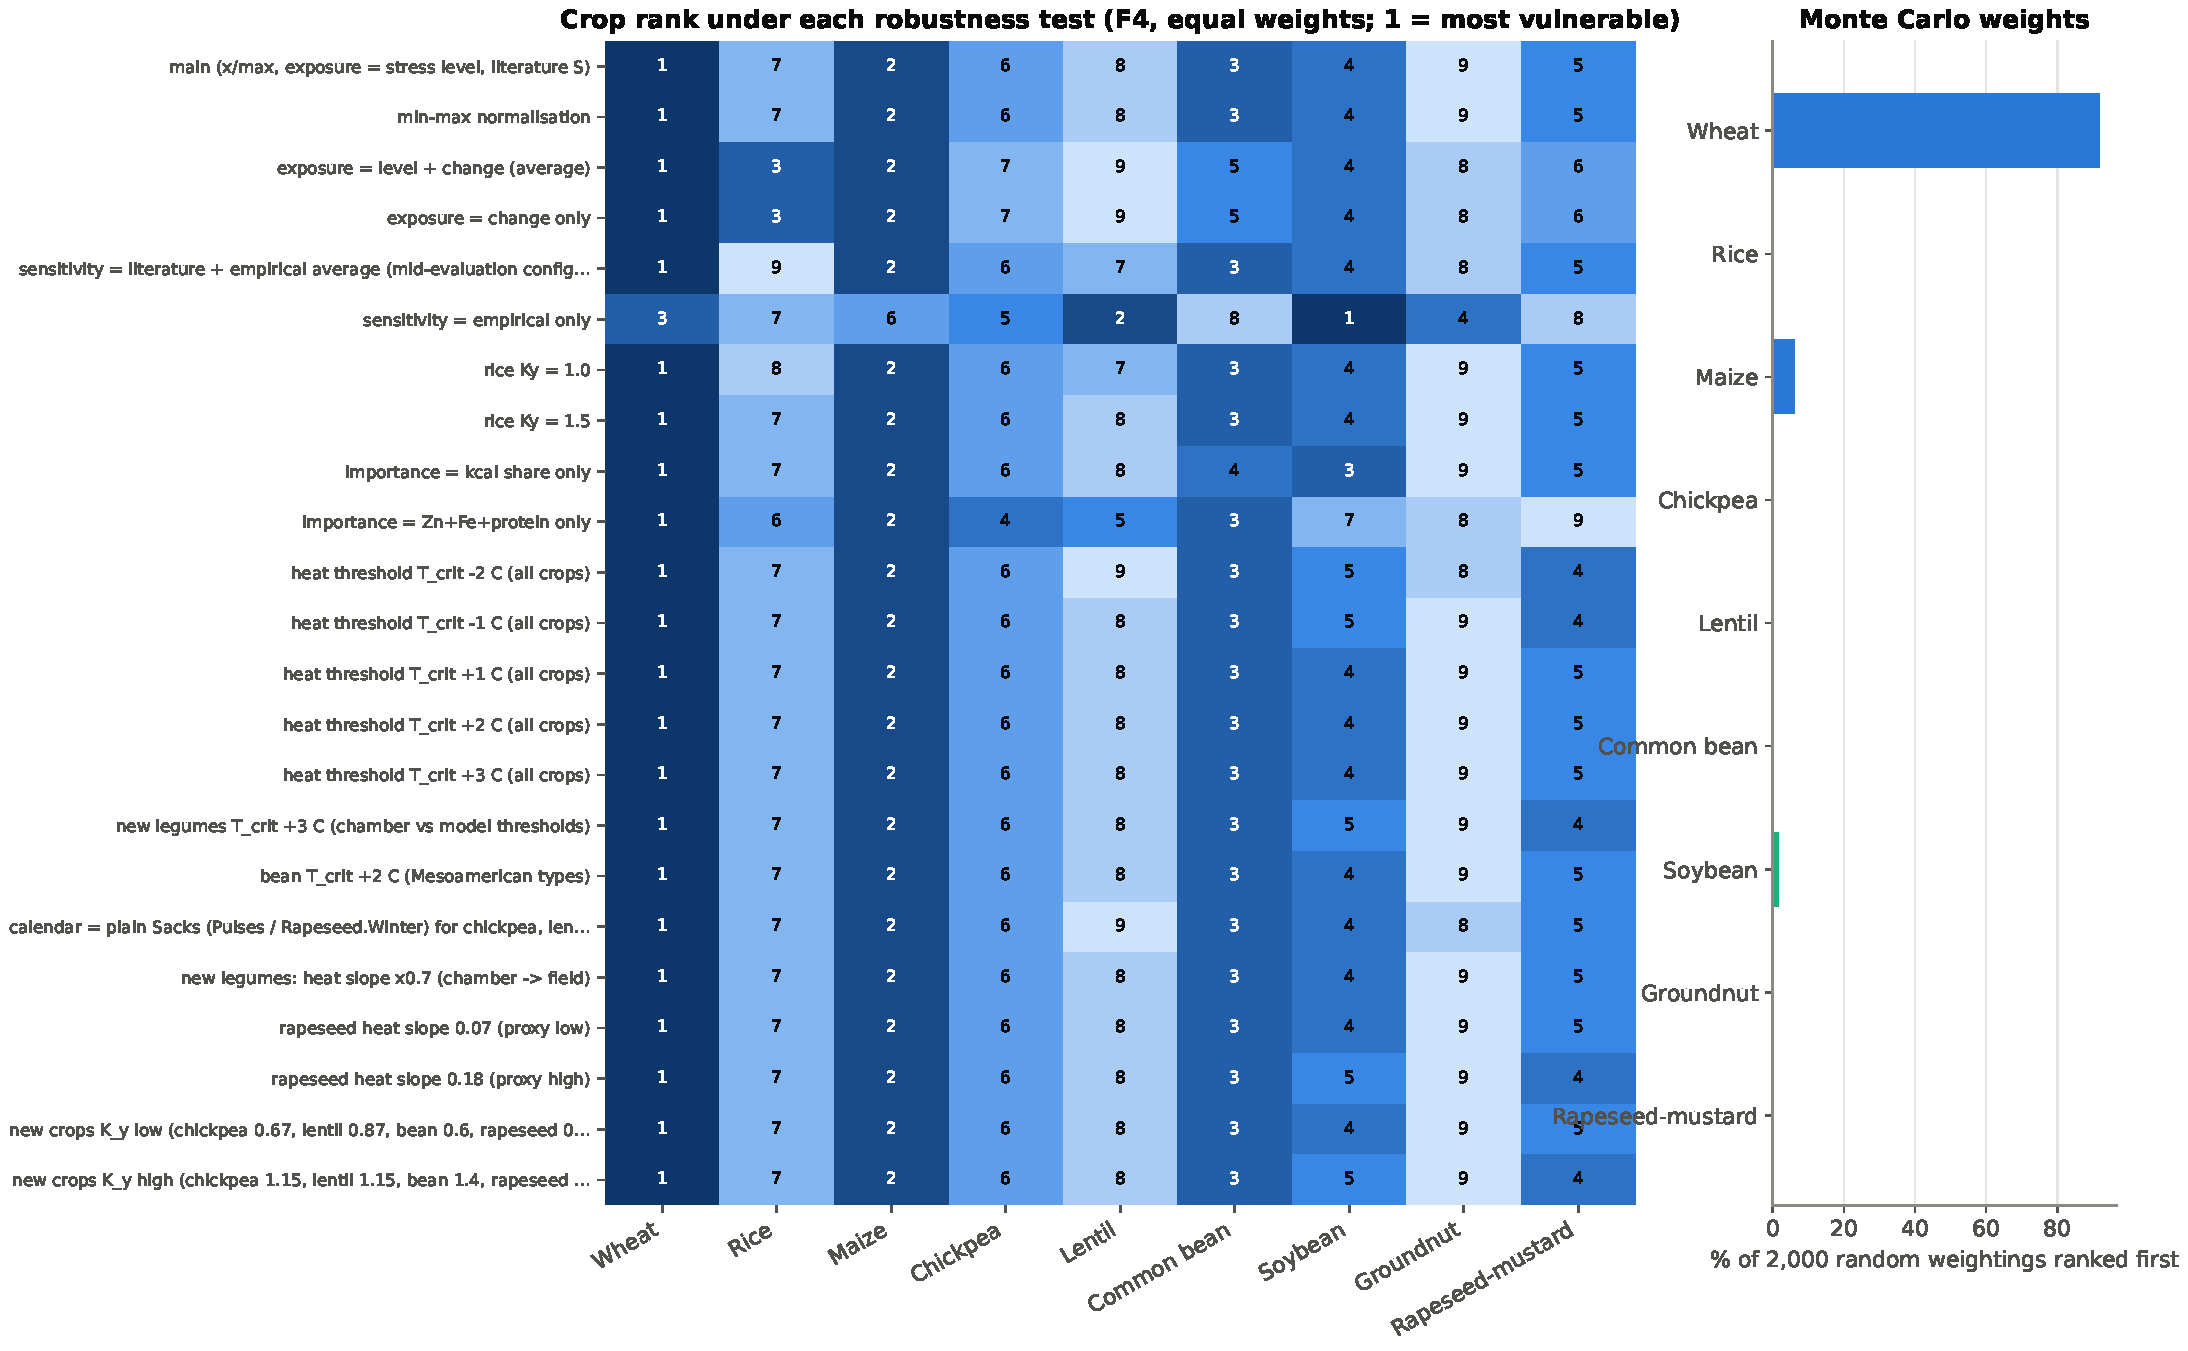
\includegraphics[width=\linewidth]{G10_robustness.pdf}
\caption{Robustness: crop ranks under each one-at-a-time test (left) and shares of first place under random
weightings (right).}\label{fig:robust}\end{figure}

\subsection{Validation against observations}
\begin{itemize}
\item \textbf{Zhao et al.\ (2017).} Against their per-degree global yield losses, the climate part of the index has
Spearman $\rho$ = \zhaoRhoClimate\ and the full index \zhaoRhoFfour. With four crops only, this is descriptive.
\item \textbf{Yield shocks, 2001--2024.} Across the \shockNpairs\ pairs, the climate part is positively
associated with how often yield fell more than one standard deviation below trend ($\rho$ = \shockRho, one-sided
permutation $p$ = \shockP).
  \begin{itemize}
  \item At the mid-evaluation, with 26 pairs, this test was null. That null result is kept on record.
  \item The nine-crop result is an association in a larger and more varied sample, not proof that the index
  predicts shocks.
  \end{itemize}
\item \textbf{Year-to-year anomalies.} The fitted climate response correlates positively with observed 2001--24
yield anomalies in \oosPos\ of \oosN\ pairs with enough data (median $r$ = \oosMedian).
\item \textbf{Future responses.} The literature and empirical future yield responses agree in sign for only
\fySameSign\% of pairs (Section~\ref{sec:futurenut}). This is a disagreement, not a validation.
\end{itemize}

\subsection{Comparison with published studies}
Section~\ref{sec:futurelit} extends this comparison to future-impact studies for all nine crops and reports where
none was found. The earlier comparison of \litN\ findings (Table~\ref{tab:lit}) is kept: \litAgree\ agree,
\litPartial\ partly agree, \litDiffer\ differ and \litOther\ are not directly comparable or add a pathway (the Ray et
al.\ row, which concerns climate-explained variability and not vulnerability, was moved here in the November audit).
These counts say how the evidence is distributed, not how accurate
the model is; several of the studies supply inputs we use (for example \citealp{deryng2014}), so agreement with them is
not independent. The disagreements are informative:
\begin{itemize}
\item \citet{lobell2011} attribute Russian wheat losses to temperature, while our monthly threshold measure sees
mainly rainfed water deficit there;
\item maize suitability studies \citep{ramirez2017} project losses in Africa where our single climate model projects
a wetter South African growing season.
\end{itemize}
Each published value is checked against its source (quote, page or table, read level) in
\file{docs/evidence/literature\_comparison\_sources.md}. Only signs and rank orders are compared, never index values with
yield percentages.

\begin{table}[p]\centering\scriptsize
\caption{Our results next to published findings (verdicts computed from our result tables by
\file{code/22\_literature\_comparison.py}).}\label{tab:lit}
\begin{minipage}{\textwidth}\centering
\adjustbox{max width=\textwidth}{\begin{tabular}{p{0.9cm}p{3.0cm}p{4.4cm}p{4.6cm}p{2.0cm}}
\toprule
 & Study & Published finding & Our comparable result & Verdict \\
\midrule
Z1 & Zhao et al. 2017 PNAS & yield change per +1 C: maize -7.4, wheat -6.0, rice -3.2, soybean -3.1 (n.s.) -$>$ maize $>$ wheat $>$ rice $>$ soybean & climate part E x S (equal weights): maize $>$ wheat $>$ soybean $>$ rice; Spearman rho with Zhao = +0.8 (n = 4) & agree (order of maize, wheat) \\
Z2 & Zhao et al. 2017 PNAS (Fig. 3) & wheat loss per +1 C: India -9.1, Russia -7.8, USA -5.5, China -2.6 \% & wheat heat exposure E\_heat: India 0.115, Russia 0.015, USA 0.015, China 0.002 & agree (heat) \\
L1 & Lobell, Schlenker \& Costa-Roberts 2011 Science & Russia wheat production about -15 \% from temperature trends & wheat-Russia F4 = 0.1315 (top pair); heat part 0.0027 vs water part 0.1288 & differ (mechanism) \\
R1 & Ray et al. 2015 Nat. Commun.; Ray et al. 2019 PLoS ONE & climate explains 32-39 \% of yield variability; rice least & rice climate part E x S = 0.0247, lowest of the four (wheat 0.1077, maize 0.1345, soybean 0.0830) & not directly comparable (different outcome) \\
D1 & Deryng et al. 2014 ERL (Table 1) & maize -10.5, wheat -10.1, soybean -6.9 \% (RCP4.5 with CO2: -4.9, +13.0, +10.8) & our conditional yield change (mean over countries, no CO2): maize -2.5 \%, wheat -3.5 \%, soybean +0.7 \% & sign agrees for maize; sign agrees for wheat; sign differs for soybean; our magnitudes smaller \\
C1 & Challinor et al. 2014 Nat. Clim. Change & $>$ 70 \% of projections show yield losses & 76 \% of our 59 pairs show a climate-driven yield loss (literature accounting); cereals only: 74 \% & agree \\
RC & Ramirez-Cabral et al. 2017 Sci. Rep. & suitable area: Africa -7 to -11 \%, South America -5 \%, India marginal areas become unsuitable & maize change in F4 2041-60 vs 1971-2000: South Africa -0.0127, Brazil +0.0019, India -0.0002 & differ \\
RP/HU & Rippke et al. 2016 Nat. Clim. Change; Hummel et al. 2018 Sci. Rep. & beans -10 \% area needing transformation in Uganda/Tanzania by the 2050s (RP); most SE African bean areas unsuitable by 2040-69, drought-driven (HU) & bean-Tanzania F4 change +0.0188; conditional yield change -17.7 \% & agree (direction) \\
Q1 & Qian et al. 2019 ERL (Table 2) & -0.8 to -5.7 \% production at +2 C with CO2 fixed (+3 to +11 \% with CO2) & rapeseed-Canada conditional yield change -3.2 \% (no CO2); flowering T\_eff change +3.1 C & agree (sign) \\
K1 & Kalra et al. 2008 Curr. Sci. & yields fall with warmer seasons: chickpea -0.53 to -3.01, mustard -0.92 to -2.01 q/ha per C & India 2041-60: chickpea T\_eff +1.3 C, yield -0.2 \%; rapeseed-mustard T\_eff +1.6 C, yield -2.2 \% & agree (sign) \\
BE/NE & Beach et al. 2019 Lancet Planet. Health; Nelson et al. 2018 Nat. Sustain. & South Asia iron availability below the recommended intake; micronutrients, not calories, are the binding constraint & India 2021-23 iron supply / requirement = 0.89 (15 \% bioavailability: 1.00); energy 1.00, protein 1.00 & agree (main requirement) \\
M1 & Myers et al. 2014 Nature & iron concentration: wheat -5.1, rice -5.2, soybean -4.1 \% (significant) & applied to India's 2021-23 iron supply shares, these declines alone would lower national iron supply by 2.2 \% (an additional pathway the index excludes) & additional pathway \\
\bottomrule
\end{tabular}
}
\par\vspace{2pt}{\footnotesize Signs and rank orders only; published values verified in docs/literature\_comparison\_sources.md; ours computed by code/22\_literature\_comparison.py.}
\end{minipage}

\end{table}
